%%%%
\section{Black Carbon}

\textbf{Black Carbon} é um nome genérico que se da aos componetes
absorvedores de luz que compoe o material particulado e é formado pela combustão
incompleta de combustíveis fósseis, biocombustível e biomassa.. 
É encontrado predominantemente na fração fina do material particulado 
e dependendo da região, representa mais da metade da massa do $MP_{2,5}$. 
Sua principal fonte em cidades são veículos automotores, 
especialmente os movidos a diesel \citep{petzold2013}. 

Exposição a \textbf{Black Carbon} causa probelmas respiratórios, cardiovasculares 
e morte prematura \citep{jacobson2014}.

%%%%
\subsection{Refletância}

Concentrações de \textbf{Black Carbon BC} foram obtidas por um 
refletômetro \textbf{Smoke Stain Refletometer, DiffusionSystem} modelo M43D, 
pertencente ao \textbf{LAPAt}.

\begin{figure}[H]
  \centering
  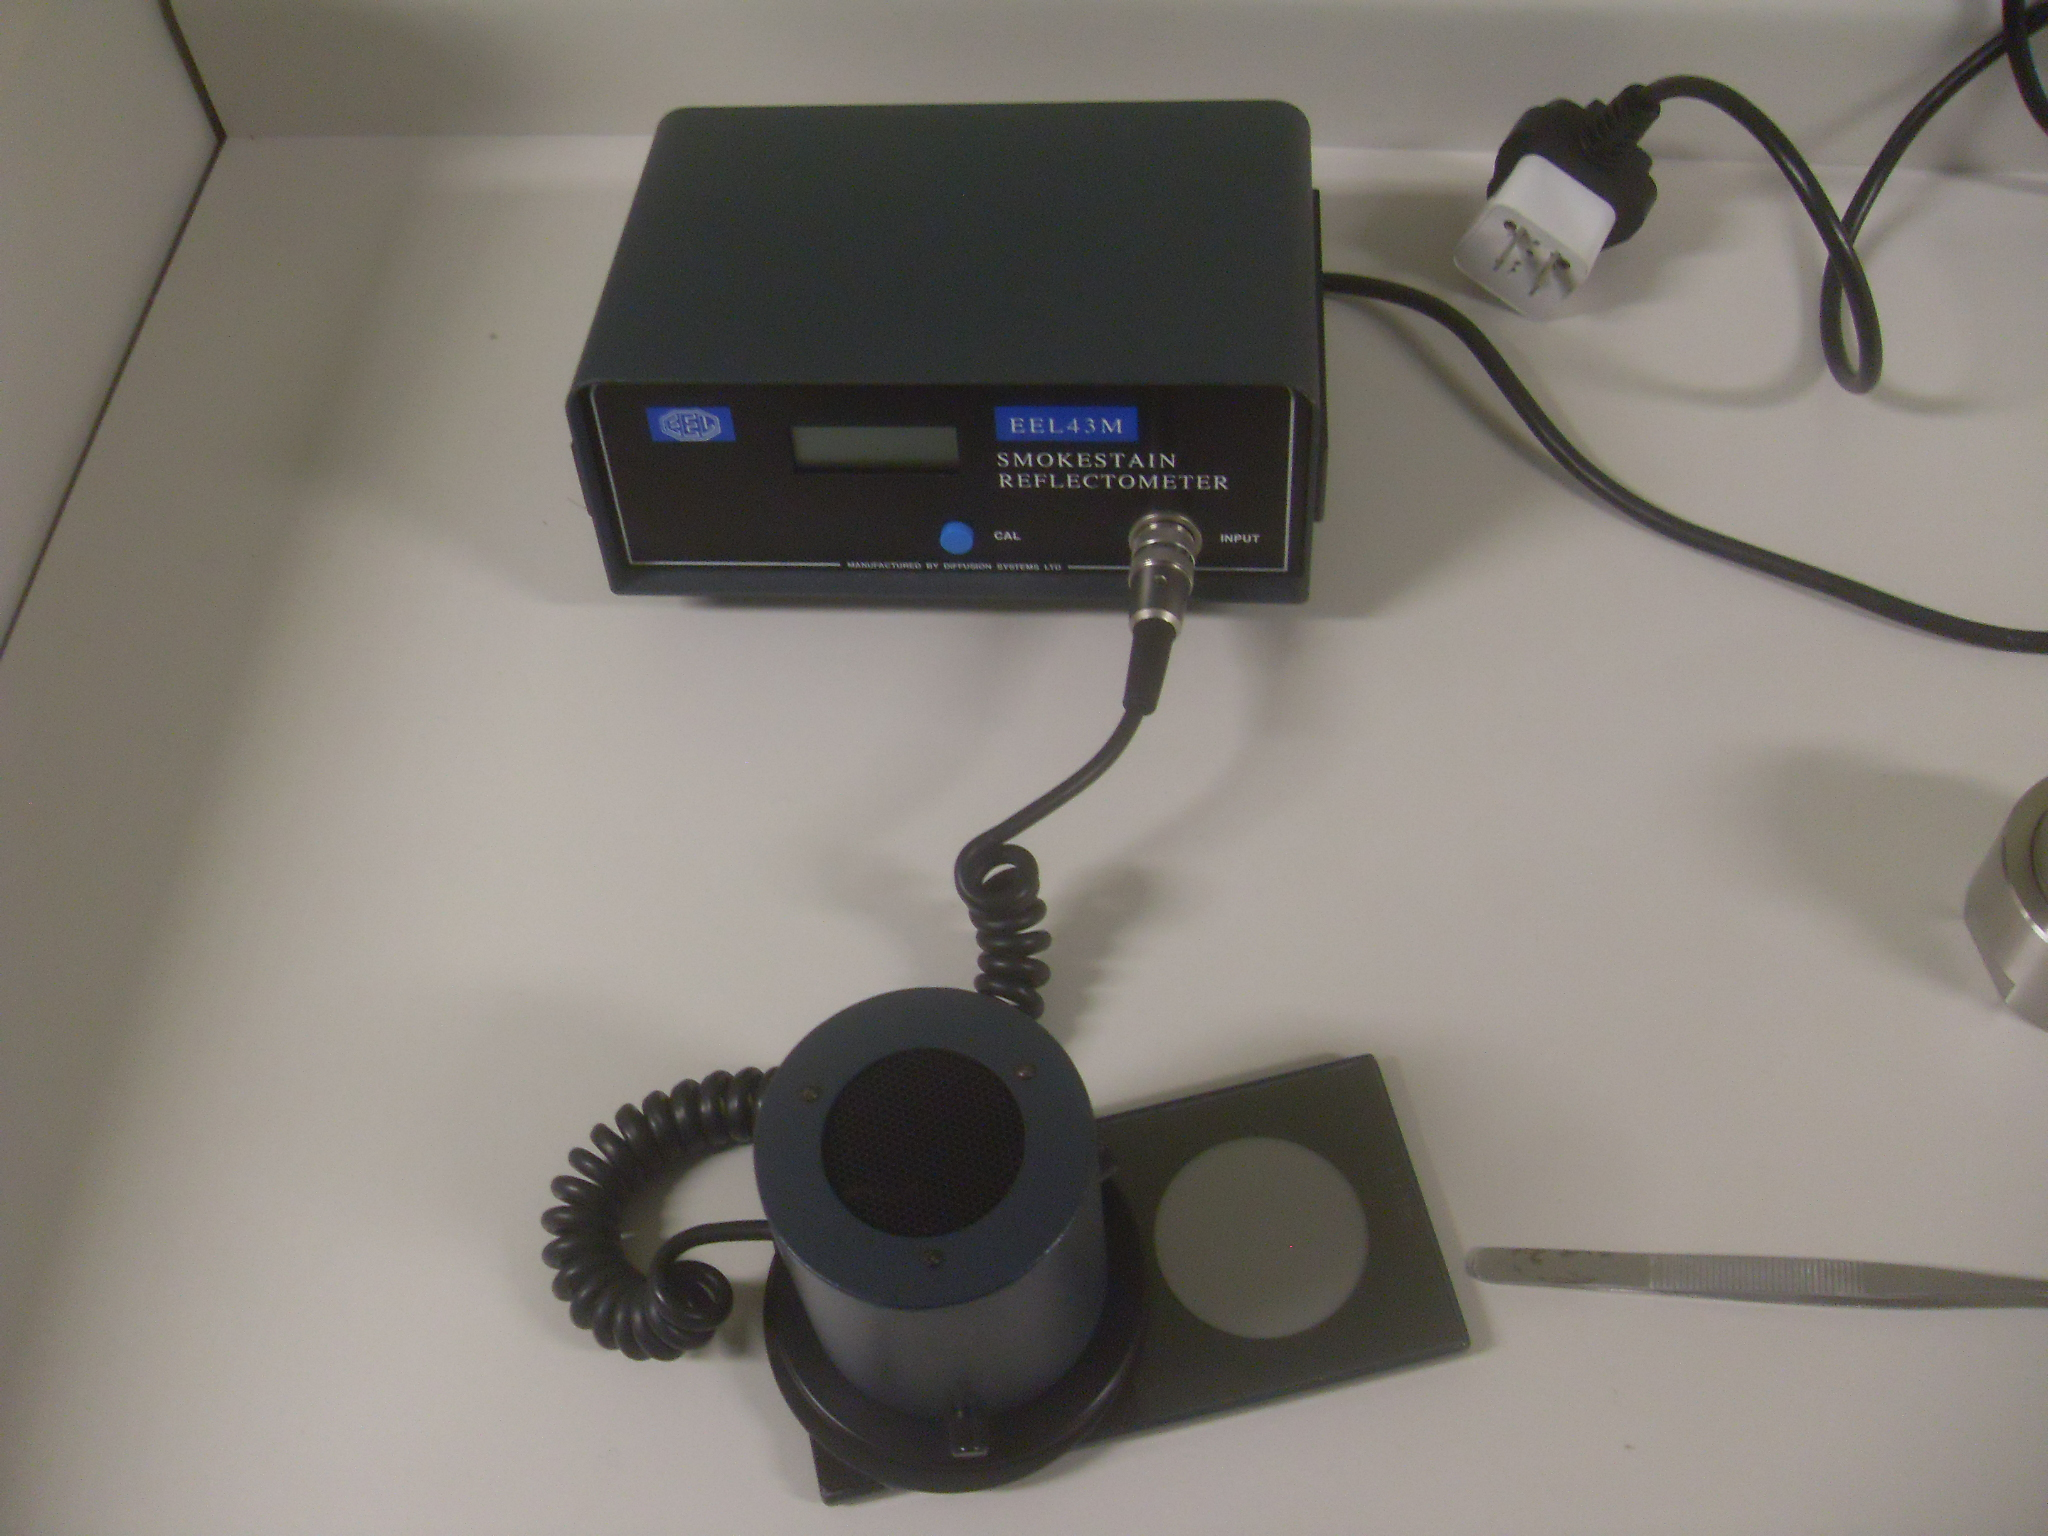
\includegraphics[width=0.5\textwidth]{../inputs/images/refletometro.jpg}
  \caption{Refletômetro \textbf{Smoke Stain Refletometer, DiffusionSystem} modelo M43D 
           e peças auxiliares de fixação do filtro \textbf{LAPAt}}
\end{figure}

A técnica baseia-se na propriedade do composto \textbf{Black Carbon} 
possuir alta seção de choque de absorção de luz na região do visível.

A radiação emitida por uma lâmpada de tungstênio reflete nas amostras, 
detectando-se o percentual de luz refletida. Este sistema é calibrado 
com amostras padrões, o que permite a determinação da concentração de $BC$
\citep{lack2014}.

Para calibração do refletômetro do \textbf{LAPAt} utilizou-se alvos padrões
tipo \textbf{monarch 21} \citep{clarke1986}. Os valores de reflêtancia 
desses filtros, bem como a massa de \textbf{Black Carbon} conhecida,
etão na tabela \ref{table:monarch21ifusp}.

\begin{table}[H]
 \centering
  \begin{scriptsize}
    \input{../outputs/CalibracaoRefletancia2007.tex}
  \end{scriptsize}
  \caption{Reflêtancia de filtros padrões tipo Monarch 21 \citep{clarke1986} 
           do \textbf{IFUSP} usados na calibração do refletometro do 
           \textbf{LAPAt} 2007 - \label{table:monarch21ifusp}}
\end{table}

O logarítimo da refletância possui relação linear com a massa.
A calibração para refletância encontra-se no gráfico da figura 
\ref{fig:mocarch21calib}. 

\begin{figure}[H]
  \centering
  \includegraphics[width=0.5\textwidth]{../outputs/CalibracaoRefletancia2007Lapat.pdf}
  \caption{Calibração refletômetro do \textbf{LAPAt} usando alvos padrões Monarch 21
          \label{fig:mocarch21calib}}
\end{figure}

%%%%
\subsection{Thermal/Optical Transmittance (TOT)}

O \textbf{Thermal/Optical Transmittance (TOT)} é um método absoluto
que mede carbono orgânico (OC) e carbono elementar (EC).
É baseado no princípio  de que diferentes tipos de partículas
compostas de carbono são convertidas para gás em diferentes temperaturas e condições
de oxidação \citep{birch1998}.

Ao aumentar a temperatura, os compostos orgânicos do filtro são volatilizados 
na atmosfera de $He$ não oxidada.
A evaporação do carbono elementar ocorre em temperaturas maiores que 
$580 \degree C$ em atmosfera de $He$ oxidada.
O sistema térmico consiste de um tubo de quartzo dentro de uma bobina aquecida, 
onde temperatura é controlada por intervalos de tempo.  

Segue-se a sequência de volatilização conforme aumento de temperatura e 
oxidação da atmosfera:

\begin{itemize}
  \item OC1: atmosfera de Hélio na temperatura ambiente $(\pm 25 \degree C)$ até $140 \degree C$
  \item OC2: atmosfera de Hélio em temperatura de $140 \degree C$ até $280 \degree C$
  \item OC3: atmosfera de Hélio em temperatura de $280 \degree C$ até $480 \degree C$
  \item OC4: atmosfera de Hélio em temperatura de $480 \degree C$ até $580 \degree C$
  \item EC1: atmosfera oxidada com temperatura de $580 \degree C$
  \item EC2: atmosfera oxidada com temperatura de $580 \degree C$ até $740 \degree C$
  \item EC3: atmosfera oxidada com temperatura de $740 \degree C$ até $840 \degree C$
\end{itemize}

O gás formado com aumento da temperatura passa por uma placa de dióxido de magnésio 
aquecida e é oxidado para dióxido de carbono, passando por um catalizador de níquel, 
que reduz o dióxido de carbono em metano $CH_4$.
O $CH_4$ é quantificado com uma detector do tipo 
\textbf{flame ionization detector (FID)}.

Durante a fase de volatilização do carbono orgânico, parte do carbono elementar
é decomposto pelo processo de pirólise. 
O sistema ótico composto por laser de $He-Ne$ com feixe de intensidade controlada, 
transmissor de fibra ótica e uma fotocélula, contabiliza o carbono elementar
decomposto nesta fase por transmitância.

O carbono elementar total é resultado da soma EC1 + EC2 + EC3 + ECP,
onde ECP é o carbono elementar formado por pirólise. 

Para análises \textbf{TOT} é necessário fazer a coleta em filtros
de quartzo, aumentando os custos e dificultando a logística das medidas, 
pois é necessário montar ponto de medida paralelos.  

Neste trabalho, coletou-se material particulado em filtros de 
quartzo para $\pm 10\%$ dos dias de amostragem e utilizou-se
dos resultados da medida de carbono elementar por \textbf{TOT} 
para inter-calibrar os resultado das medidas de refletância. 
